
\documentclass[ms.tex]{subfiles}
\begin{document}
\renewcommand\theequation{\thesection\arabic{equation}}
\renewcommand\thefigure{\thesection\arabic{figure}}
\setcounter{equation}{0}
\setcounter{figure}{0}

\section{The Yield-Outflow Degeneracy}
\label{sec:yield_outflow_degeneracy}

\begin{figure*}
\centering
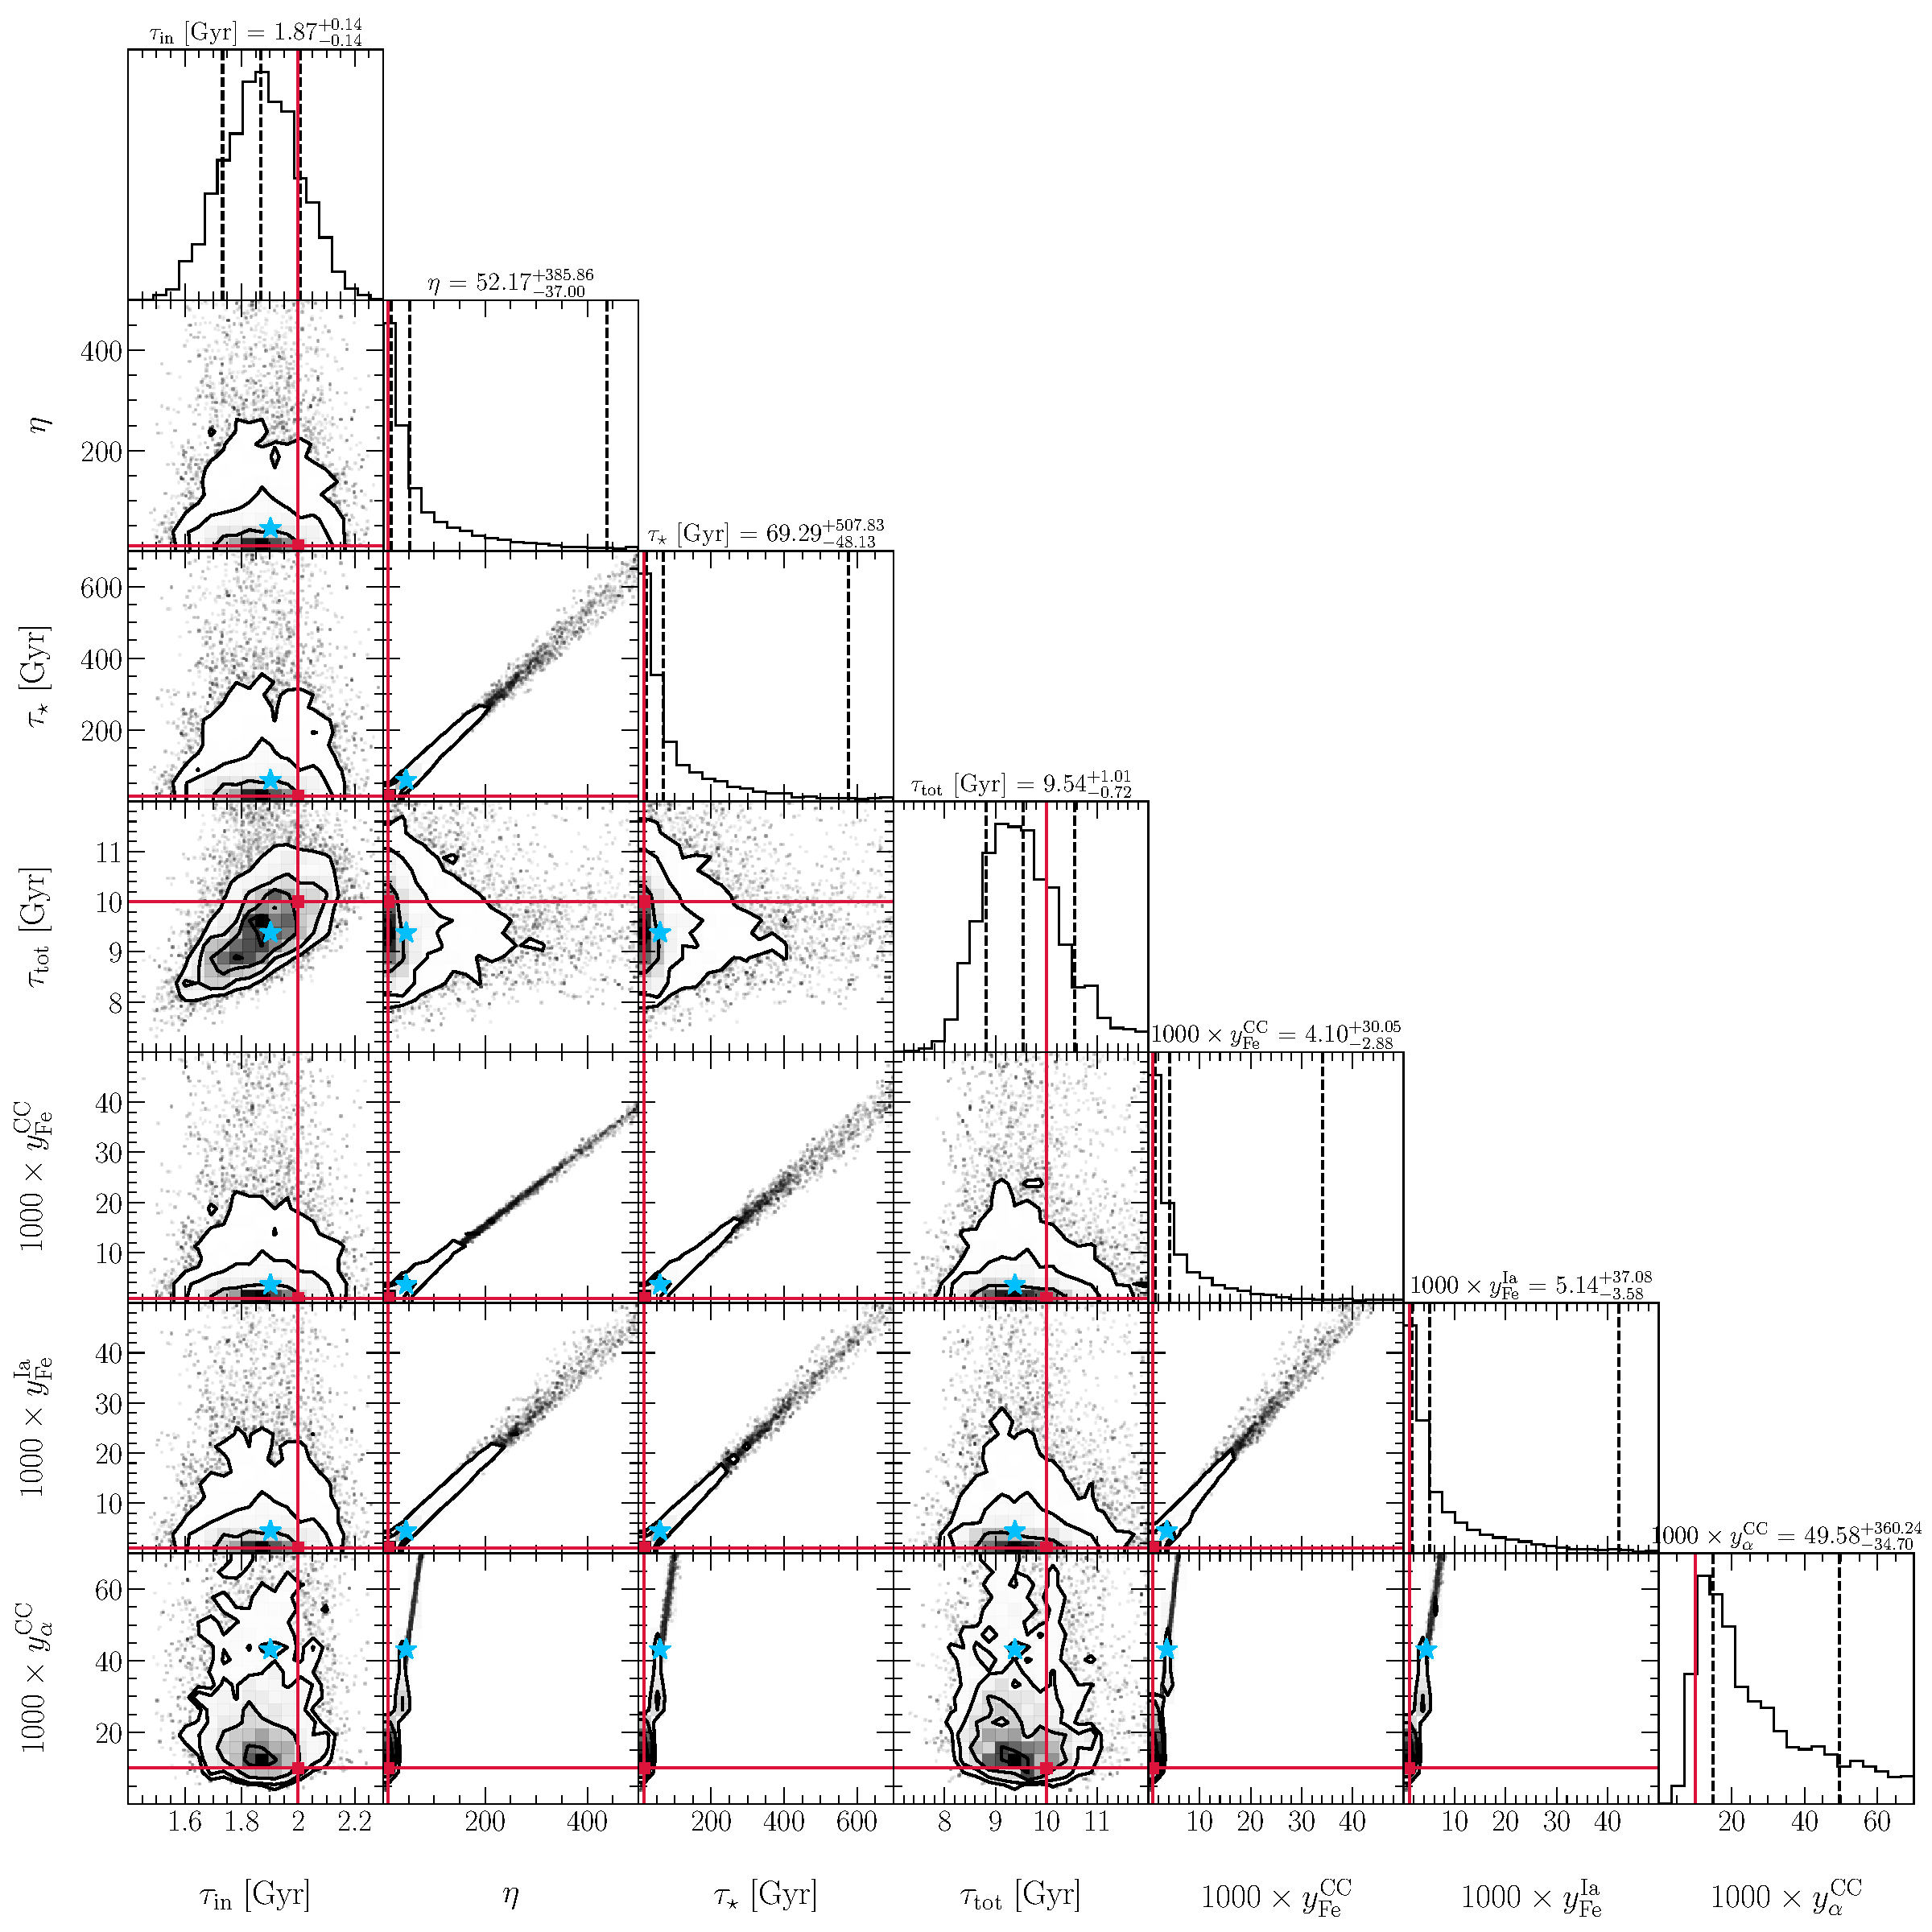
\includegraphics[scale = 0.4]{degeneracy_25k6.pdf}
\caption{
The same as Fig.~\ref{fig:fiducialmock}, but with the alpha element yield from
massive stars~\yacc~as an additional free parameter.
Motivated both by theoretical models of nucleosynthesis in massive stars and
the convenience for scaling up or down, we have adopted~$\yacc \equiv 0.01$
in this paper to set the scale of this degeneracy.
}
\label{fig:degeneracy}
\end{figure*}

\begin{itemize}

	% \item As discussed in~\S~\ref{sec:onezone:yields}, there is a
	% degeneracy between the absolute scale of nucleosynthetic yields and the
	% strength of outflows in GCE models.
	\item Under the instantaneous recycling approximation, early work in GCE
	demonstrated that galaxies with ongoing accretion of metal-poor gas
	reached an equilibrium metal abundance in which the newly produced metal
	mass is balanced by losses to star formtion and, if present, outflows
	(e.g.~\citealp{Larson1972}, and more recently~\citealp{Weinberg2017}).
	These ``open-box'' models offered a simple solution to the G-dwarf problem
	which plagued the ``closed-box'' models of GCE, whereby the frequency of
	super-solar metallicity stars was severely over-predicted (see the review
	in, e.g.,~\citealp{Tinsley1980}).

	\item These results were corroborated by~\citet{Dalcanton2007}, who argued
	that metal-enriched outflows are the only mechanism which can
	significantly reduce effective yields from SNe.
	However, recent theoretical explorations of SN explosions propose that
	many massive stars collapse directly to form black holes at the end of
	their lives as opposed to exploding as CCSNe (e.g.~\citealp{Ertl2016,
	Sukhbold2016}; see also discussion in~\citealp{Griffith2021}).
	This challenges the interpretation of~\citet{Dalcanton2007}, instead
	suggesting that SN yields are perhaps~\textit{intrinsically} lower and
	consequently may not require adjusting with metal-enriched outflows to
	alter effective yields.
	Observationally, it is feasible to constrain relative but not absolute
	yields.
	For example, the two-process model explored by~\citet{Weinberg2019,
	Weinberg2021} in APOGEE~\citep{Majewski2017} and by~\citet*{Griffith2019}
	and~\citet{Griffith2022} in GALAH~\mbox{\citep{DeSilva2015, Martell2017}}
	quantifies the median trends in abundance ratios relative to Mg along the
	high- and low-alpha sequences to disentangle the relative contributions of
	prompt and delayed nucleosynthetic sources to various elements.
	Abundance ratios can also be derived from individual supernova remnants as
	in, e.g.,~\citet*{Holland-Ashford2020}, but these investigations cannot
	constrain absolute yields.

	\item Furthermore, there are many parametrizations of outflows in the
	literature. Recently,~\citet{delosReyes2022} modelled the evolution of the
	Sculptor dwarf spheroidal by letting the outflow rate instead be linearly
	proportional to the SN rate~$\dot{N}_\text{II} + \dot{N}_\text{Ia}$.
	\citet*{Kobayashi2020} constructed a model for the Milky Way in which
	outflow-driving winds develop in the early phases of evolution, but die
	out as the Galaxy grows.
	Based on theoretical models suggesting that the re-accretion timescales
	of metals ejected from the Milky Way disk are short ($\sim$100 Myr;
	\citealp{Melioli2008, Melioli2009, Spitoni2008, Spitoni2009}), some
	authors even neglect outflows entirely when modelling the Milky Way (e.g.
	\citealp{Spitoni2019, Spitoni2021}, and the recently released publicly
	available GCE code~\textsc{GalCEM}; Gjergo et al. 2022, in prep).
	This argument is, however, at odds with the empirical result that
	multi-phase galaxy-scale outflows are ubiquitous around galaxies of a broad
	range of masses (see, e.g., the recent review in~\citealp{Veilleux2020}).
	Furthermore, mesaurements of the deuterium abundance (\citealp{Linsky2006};
	~\citealp*{Prodanovic2010}) and the~$^3$He/$^4$He ratio~\citep{Balser2018}
	in the local ISM indicate near-primordial values.
	This indicates that much of the gas in the Galaxy has not been
	processed by stars, further suggesting that outflows can sweep up ambient
	ISM which can then be replaced by unprocessed baryons~\citep{Weinberg2017b,
	Cooke2022}.
	Although it is possible that much of the deuterium could be depleted
	onto dust grains (\citealp{Romano2006};~\citealp*{Steigman2007}), the
	same cannot be said of~$^3$He or~$^4$He.

	\item Suffice it to say that the community has settled on neither the
	proper parametrization nor the importance of outflows in GCE models.
	As discussed in~\S~\ref{sec:onezone},
	the strength of outflows (i.e. the value of~$\eta$ in this work) is
	strongly degnerate with the absolute scale of effective nucleosynthetic
	yields because the latter is the primary source term in describing the
	enrichment rates while the former is the primary sink term.

	\item In this paper, we have applied our fitting method on an assumed scale
	in which the alpha-element yield from massive stars is defined to
	be~$\yacc \equiv 0.1$.
	As mentioned in~\S~\ref{sec:onezone}, this value is somewhat informed by
	nucleosynthesis theory in that massive star evolutionar models
	\citep{Nomoto2013, Sukhbold2016, Limongi2018} typically predict
	IMF-averaged O yields of~$y_\text{O}^\text{CC} = 0.005 - 0.015$.
	While massive star explodability and the black hole landscape
	\citep[e.g.][]{OConnor2011, Pejcha2015, Ertl2016, Sukhbold2016} can produce
	lower values of~\yacc~by factors of~$\sim2 - 3$~\citep{Griffith2021},
	values lower by an order of magnitude or more can be achieved if a
	significant fraction of SN ejecta are immediately lost to a hot outflow.
	This is a necessary addition to models which assume~$\eta = 0$ as otherwise
	unphysically high metal abundances will arise.
	There is some observational support for this scenario in that galactic
	outflows have been seen to be significantly more metal-rich than the ISM of
	the host galaxy (\citealp*{Chisholm2018};~\citealp{Cameron2021}), but the
	metallicities are not as high as the SN ejecta themselves and cold-phase
	material is generally observed in outflows as well (e.g., in M82,
	\citealp{Lopez2020}; see also the recent review by~\citealp{Veilleux2020}).

	\item We now quantify the strength of the yield-outflow degeneracy by
	introducing~\yacc~as an additional free parameter in our fit to our
	fiducial mock sample described in~\S~\ref{sec:mocks:fiducial}.
	Otherwise, we follow the exact same procedure to recover the known
	evolutionary parameters of the mock as discussed
	in~\S\S~\ref{sec:fitting} and~\ref{sec:mocks:fiducial_fit}.
	Fig.~\ref{fig:degeneracy} illustrates the results of this procedure in the
	form of the ``corner-plot'' with the marginalized likelihood distributions
	along the diagonal and the 2-dimensional cross-sections of the likelihood
	function below the diagonal.
	As expected, there are extremely strong degeneracies in all yields with
	one another and with the outflow parameter~$\eta$.
	Additionally, there is a degeneracy between the SFE timescale~$\tau_\star$
	and the yields which arises because the position of the ``knee'' in
	the~\afe-\feh~plane can be fit with either a high-yield and slow star
	formation or a low yield and high star formation.
	The strength of these degeneracies is espeically striking because this is
	mock data drawn from a simple model with known evolutionary parameters.

	\item In detail, this degeneracy arises whenever a parameter influences
	the position or shape of the evolutionary track in the~\afe-\feh~diagram
	or the centroid of the MDF.
	The infall timescale~$\tau_\text{in}$ and the total duration of star
	formation~$\tau_\text{tot}$ are unaffected by this degeneracy because they
	meet this criterion (see discussion in~\S~\ref{sec:mocks:fiducial}).
	Regardless of the choice of yields and of the parameters~$\eta$ and
	$\tau_\star$, the shape of the MDF is constrained by a sufficiently large
	sample, allowing precise derivations of these timescales from our fitting
	method.
	By determining the duration of star formation in this manner, this may
	open a new pathway to deriving quenching times for now quiescent dwarf
	galaxies and stellar streams orbiting local group spirals such as the
	Milky Way and Andromeda (see discussion in~\S~\ref{sec:mocks:variations}).

\end{itemize}

\end{document}

